\phantomsection\section*{\centering CHƯƠNG 3. THUẬT TOÁN}
\addcontentsline{toc}{section}{\numberline{}CHƯƠNG 3. THUẬT TOÁN}
\setcounter{section}{3}
\setcounter{subsection}{0}
\setcounter{figure}{0}
\setcounter{table}{0}
Đây \cite{stein2011fourier} là phần sinh viên tự phát triển như xây dựng thuật toán, xây dựng chương trình, mô phỏng, tính toán, thiết kế, chạy thử kết quả... \cite{howell2016principles}
\subsection{Cách chèn ảnh}
\begin{figure}[H]
    \centering
    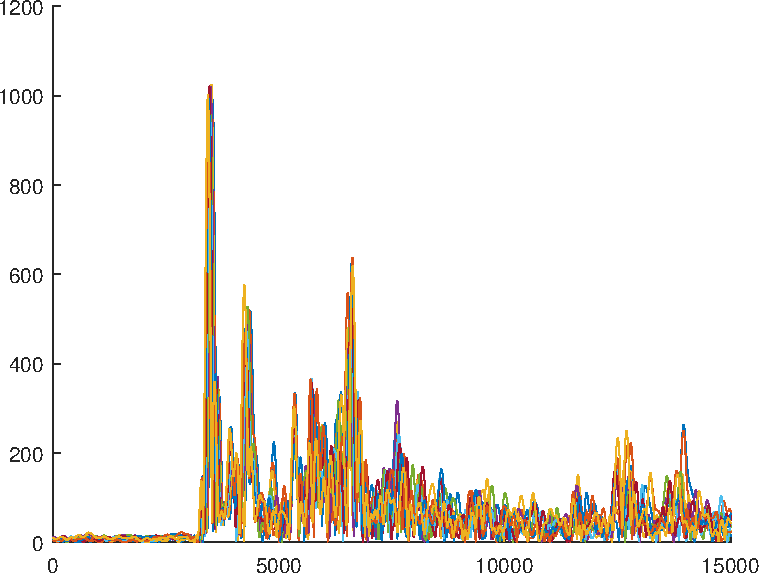
\includegraphics[width=0.75\textwidth]{Images/signal.pdf}
    \caption[Sơ đồ khối của hệ thống]{\textit{\fontsize{12pt}{0}\selectfont Sơ đồ khối của hệ thống}}
    \label{hinh31}
\end{figure}
Hình \ref{hinh31} là ví dụ về cách chèn ảnh. Nên export ảnh từ matlab theo câu lệnh: \textbf{exportgraphics(gcf, 'myfigure.pdf', 'ContentType', 'vector');} (chỉ matlab phiên bản 2021b trở lên mới được) nhưng nó xịn như hình trên. Lưu ý chú thích của hình vẽ được đặt ngay dưới hình vẽ. Tất cả các hình vẽ phải được đề cập đến trong phần nội dung và phải được phân tích và bình luận giống mình đang làm thế này nhé hihi :)

\subsection{Cách tạo bảng}
\begin{table}[H]
    \centering
    \caption[Kết quả thí nghiệm]{\textit{\fontsize{12pt}{0}\selectfont Kết quả thí nghiệm}}
    \begin{tabularx}{0.75\textwidth}{
        |>{\centering\arraybackslash}s
        |>{\centering\arraybackslash}a
        |>{\centering\arraybackslash}a
        |>{\centering\arraybackslash}s|
        }
        \hline
        \bfseries Lần thí nghiệm & \bfseries Điện áp đo được (mV) &\bfseries Điện áp tham chiếu (mV)& \bfseries Sai lệch (\%)\\\hline
        1&&&\\\hline
        2&&&\\\hline
        3&&&\\\hline
    \end{tabularx}
    \label{bang31}
\end{table}
Bảng \ref{bang31} là ví dụ về cách tạo bảng. Lưu ý chú thích của bảng được đặt ở trước bảng. Tất cả các bảng biểu phải được đề cập đến trong phần nội dung và phải phân tích và bình luận giống như mình đang làm nhé hehe :)

\subsection{Cách viết phương trình}
\begin{equation}
    \label{pt31}
    F(x) = \int^a_b \frac{1}{3}x^3
\end{equation}
Phương trình \ref{pt31} là ví dụ về phương trình tích phân.

Thử phương trình khác 
\begin{equation}
    \label{pt32}
    x[t_n] = \frac{1}{\sqrt{n}} \sum_{k=0}^{N-1}[f_k]
\end{equation}
Phương trình \ref{pt32} là phương trình biến đổi Fourier
\subsection{Cách viết định nghĩa, định lý, hệ quả, bổ đề...}
Định lý lấy mẫu Nq-shannon là một định lý được sử dụng trong lĩnh vực lý thuyết thông tin đặc biệt là trong viễn thông và xử lý tín hiệu 
\begin{theorem} % Định lý
    \label{dlNq}
    Một hàm số tín hiệu  $x(t_n)$ không chứa bất kỳ thành phần tần số nào lớn hơn hoặc bằng 1 giá trị $f_m$ có thể biểu diễn chính xác bằng tập các giá trị của nó với chu kỳ lấy mẫu $T = 1/(2f_m)$.
\end{theorem}
Định lý \ref{dlNq} thường được gọi đơn giản là định lý lấy mẫu 
\begin{corollary}
    Một người có thể làm được thì sẽ nghĩ mình làm đư
\end{corollary}
\begin{lemma}
    Một người có thể làm được thì sẽ nghĩ mình làm đư
\end{lemma}
\begin{defn}
    \label{defn}
    Một người có thể làm được thì sẽ nghĩ mình làm đư
\end{defn}
Định nghĩa \ref{defn} được nhắc tới như là tiếng gọi hoang rã từ nơi không người
\cleardoublepage